\hypertarget{chap:method}{\chapter{Method}}\label{method}
In this section, we introduce our methods for improving the accuracy of sentiment classification task on \hyperref[sec:sst]{Stanford Sentiment Treebank dataset with binary setting}.
In search of new improvements, we have tried three different approaches:
\begin{description}
\item[\deschyperlink{sec:VTtree}{Utilizing local syntactic information at each node of Recursive Neural Networks}] The first approach is mainly based on the success of Tag Embeddings Recursive Neural Networks~\cite{tag-embedding-rnn}.
In this paper, the authors parameterized the composition functions at each parse tree's node with respect to the grammar rule expanding that node.
By doing so, the authors were able to not only efficiently improve the performance of RNTN (Socher, 2013)~\cite{socher2013recursive} (from \(85.4\%\) to \(87.7\%\) accuracy) but also use much smaller number of parameters in their models \((54K)\) compared to that of RNTN \((108K)\)~\cite{tag-embedding-rnn}.
Given the success of \hyperref[sec:treelstm]{Tree-LSTM models}, we hypothesized that by parameterized the composition functions of a Tree-LSTMs unit at a node with respect to the grammar rule expanding that node, we can improve the performance of Tree-LSTMs (in the same way how this method improves RNTN).

\textbf{This approach was later proven to be unsuccessful}, so we tried two more different approaches.

\item[\deschyperlink{sec:Glove-Amazon}{Transfer Learning by retraining Glove on Amazon Reviews dataset}] \label{movie-hypothesis} There are many words (e.g. "B-rated", "Batman", "Nolan", "cartoonlike") which rarely appears in regular documents but more often in movie reviews.
We hypothesized that by training word embeddings of review documents, especially movie or book reviews, we can capture more rare words and also the different way people use words (or different word relationships) to express their opinions on movies or books.
For archiving these purposes, we retrained Glove vectors~\cite{glove} on part of  \hyperref[sec:amazon]{Amazon Reviews dataset}.
This new Glove word vectors was named Glove Amazon.
For evaluating Glove Amazon, we replaced the Glove Common Crawl\footnote{Common Crawl (840B tokens, 2.2M vocab, cased, 300d vectors, 2.03 GB download) publicly available at \url{https://nlp.stanford.edu/projects/glove/}} with Glove Amazon for initializing Tree-LSTMs' word embedding layer.

\textbf{In spite of being a simple method, Glove Amazon dramatically improves Tree-LSTMs performance.}
This is our first successful method for transfer learning from document-level (Amazon Reviews) to sentence-level labeled dataset (Stanford Sentiment Treebank).
Inspired by this approach, we cooperated it into the development of our next approach.

\item[\deschyperlink{sec:CNNtree}{Combining Recursive Neural Networks with Convolution Neural Networks}] \label{conv-tree-benefits} Based on our discussion on tree-structured versus sequential network architects (Sec.\ref{sec:tree-discuss}) and the benefits of using convolution layer (Sec.\ref{kim-cnn}), we combined Convolution Neural Networks with Tree-LSTM and \hyperref[sec:lstm]{sequential LSTM}.
We hypothesized that the convolution layer will help Tree-LSTMs to mitigate the problem of lacking local context and weak feature capturing at leaf nodes (Sec.\ref{sec:tree-discuss}).
Additionally, using Tree-LSTM to combine the feature maps produced by convolution layer is better than max-over-time pooling layer (Sec.\ref{kim-drawback}).
The increased model complexity can lead to over-fitting.
We tackled this risk by unsupervised pre-training the models on the large Amazon Reviews dataset using methods described in Sec.\ref{sec:unsupervised-pretrain}.
Based on the success of Glove Amazon, we expected that the unsupervised pre-training process (on Amazon Reviews) help the models to capture not only generic language features but also specific knowledge about Film industry and human culture (Sec.\ref{sec:nlm}).

With this approach, \textbf{we was able to archive state-of-art\footnote{July, 2017} performance on Stanford Sentiment Treebank}.
\end{description}


\hypertarget{sec:VTtree}{\section{Utilizing local  syntactic information at each node of Recursive Neural Networks}}\label{sec:VTtree}
\subsection{Model description}

\begin{figure}[H]
    \centering
    % 
\includegraphics[width=0.8\linewidth]{figure/vtgrusummary.pdf}
    \begin{tikzpicture}
    \node (input)[io]{input};
    \node (emb)[process, right of=input, xshift=2cm, text width=2cm]{Embedding Layer};
    \node (tetreegru)[process, right of=emb, xshift=2cm, text width=3cm]{TE Tree-GRU};
    \node (outputlayer)[process, right of=tetreegru, xshift=2cm, text width=2cm]{Output Layer};
    \node (output)[io, right of=outputlayer, xshift=2cm]{sentiment};
    
    \draw [arrow](input)--(emb);
    \draw [arrow](emb)--(tetreegru);
    \draw [arrow](tetreegru) -- (outputlayer);
    \draw [arrow](outputlayer) -- (output);
    \end{tikzpicture}
    \caption[TE Tree-GRU overview]{TE Tree-GRU overview}
    \label{fig:vtgrusummary}
\end{figure}

\subsubsection{Embedding layer}\label{sec:embedding}
Embedding layer is a lookup table that converts input data (such as text) into its vector representation. Word embedding layer parameters are its embedding matrix $M  \in \mathbb{R}^{n \times d}$, where $n$ and $d$ are vocabulary size and embedding vector dimension, respectively. In practical, an embedding layer also comes with a vocabulary-index lookup table, which maps words with indexes, which has vector representation corresponding to the row in word embedding matrix.

The following steps are required once for each experiment:
\begin{itemize}
    \item Build vocabulary-index lookup table
    \item Init/Load word embedding matrix corresponding to vocabulary-index table
    \item Convert every sentence in dataset into indices using vocabulary-index table
\end{itemize}
Usually, indices are kept as dataset. Raw dataset (such as readable words) are discarded to free up memory. For each mini-batch, we use indices to look up word representation vector from embedding matrix. Embedding matrix represents of each sentence in dataset are not saved and needed look-up every mini-batch for the following reason.
\begin{itemize}
    \item Saved embedding matrix for each data sentences cost more memory than saving only indices and look-up in embedding layer.
    \item Embedding matrix contains trainable parameters and being updated every iteration.
\end{itemize}

Fig.\ref{fig:embeddinglayer} illustrates embedding layer component and describes the process of convert raw data sentence into its word representation.

\begin{figure}[H]
    \centering
    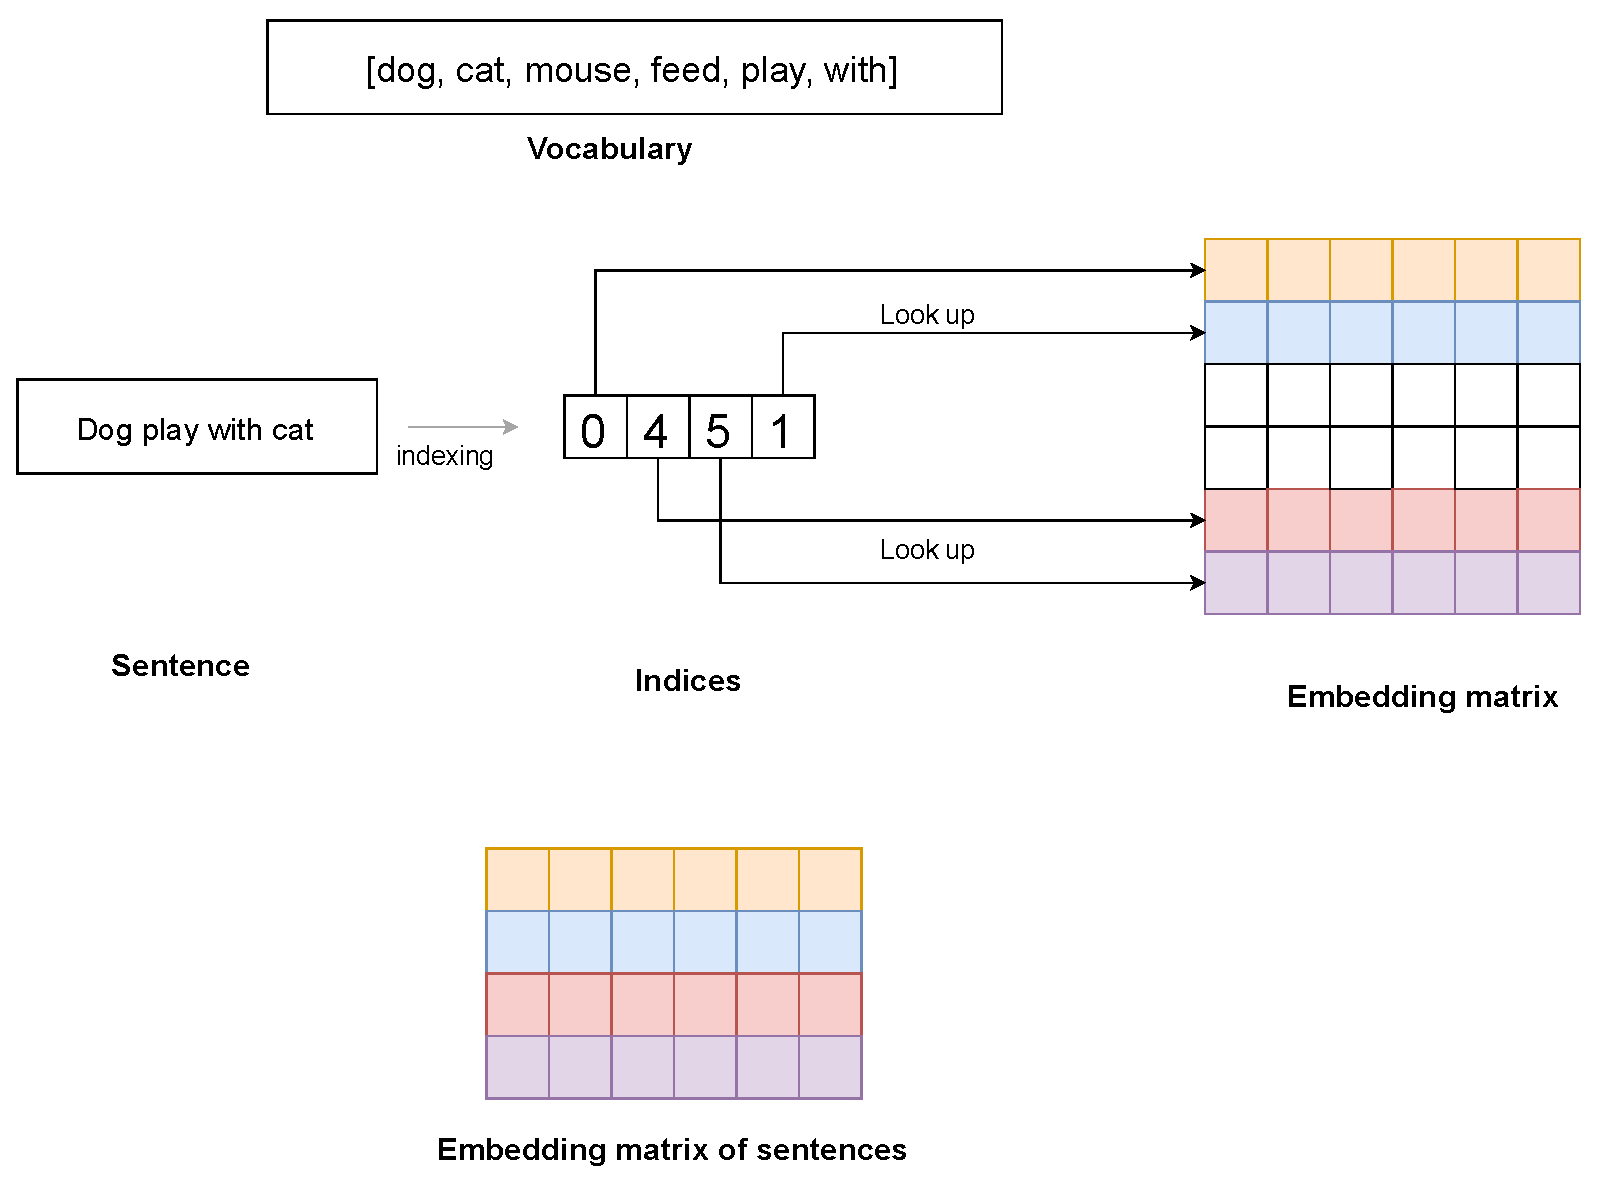
\includegraphics[width=0.9\linewidth]{figure/embeddinglayer.pdf}
    \caption[Overview of embedding layer]{Overview of Embedding Layer}
    \label{fig:embeddinglayer}
\end{figure}



\subsubsection{TE-Tree-GRU}
We applied both tree structure network and recurrent structure in our model.
To compose the vector presentation for a node, the models use information from that node and it child nodes (if it has any), we applied recurrent network over the the node and all its child nodes.
The hidden state of the last Recurrent Neural Network timestep is viewed as a vector presentation of the node. 
Recursively, the vector presentation of this node is an input for its parent node.
For recurrent unit, we chose \hyperref[sec:GRU]{Gated Recurrent Unit (GRU)}~\cite{cho2014learning}.
GRU transition equations used in our implementation are describe in Eq.\ref{eq:gru}.

\begin{equation}
\label{eq:gru}
\begin{aligned}
&r = sigmoid(W_{ir} x + b_{ir} + W_{hr} h + b_{hr}) \\
&i = sigmoid(W_{ii} x + b_{ii} + W_{hi} h + b_{hi}) \\
&n = \tanh(W_{in} x + b_{in} + r * (W_{hn} h + b_{hn})) \\
&h' = (1 - i) * n + i * h\\
\end{aligned}
\end{equation}

\subsubsection{Constituency TE-Tree-GRU} \label{sec:VTtreeConstituency}
For each node which has at least one child, we sorted the child nodes according to its relative position in the sentence. 
For any child nodes, presentation vector \(k\), embedding vectors of POS-tag and its parent node POS-tag are inputs for the GRU timestep. 
We put the parent node at the end of GRU chain. We took hidden state of the last GRU timestep as vector presentation \(k\) for the parent node. 
A node with it child nodes and its composition process is demonstrated in Fig.\ref{fig:treecp}, and Fig.\ref{fig:cvtgru} respectively. 
For leaf nodes, embedding vectors of word and POS-tag are inputted into a GRU cell and got hidden state \(h\) as vector presentation \(k\) for leaf node as Fig.\ref{fig:gruleaf}.
\begin{figure}[H]
    \centering
    % 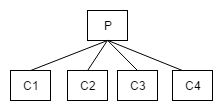
\includegraphics[width=0.5\linewidth]{figure/treecp}
    \begin{tikzpicture}
    \node[process]{P}
    child { node[process] {C1}}
    child { node[process] {C2}}
    child { node[process] {C3}}
    child { node[process] {C4}}
    ;
    \end{tikzpicture}
    \caption[A sub tree with parent and children node]{A sub tree with parent and children node}
    \label{fig:treecp}
\end{figure}

\begin{figure}[H]
    \centering
    % 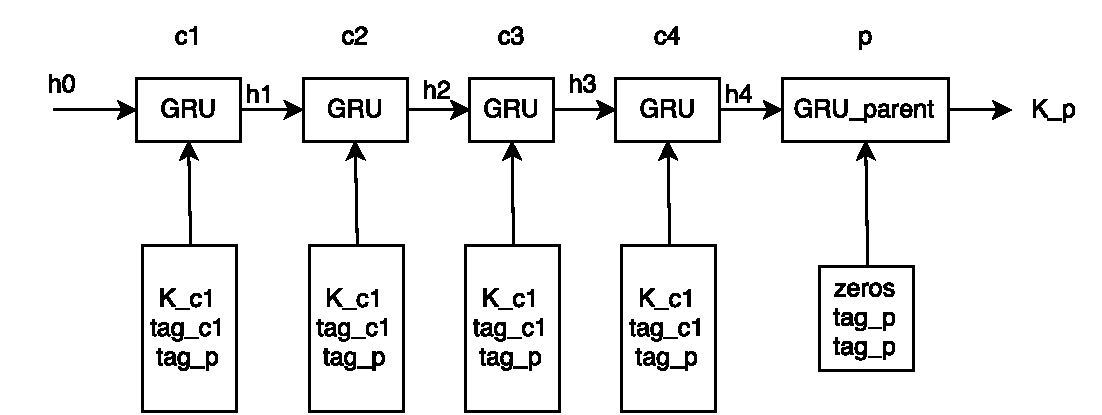
\includegraphics[width=0.9\linewidth]{figure/cvtgru}
    \begin{tikzpicture}
\node(start)[io]{};
\node(gru1)[process, right of=start, xshift=1cm]{$GRU$};
\node(gruin1)[process, below of=gru1, yshift=-1cm, text width=1cm ]{$k_{c1}$ $tag_{c1}$ $tag_{p}$};

\node(gru2)[process, right of=gru1, xshift=1cm]{$GRU$};
\node(gruin2)[process, below of=gru2, yshift=-1cm, text width=1cm ]{$k_{c2}$ $tag_{c2}$ $tag_{p}$};

\node(gru3)[process, right of=gru2, xshift=1cm]{$GRU$};
\node(gruin3)[process, below of=gru3, yshift=-1cm, text width=1cm ]{$k_{c3}$ $tag_{c3}$ $tag_{p}$};

\node(gru4)[process, right of=gru3, xshift=1cm]{$GRU$};
\node(gruin4)[process, below of=gru4, yshift=-1cm, text width=1cm ]{$k_{c4}$ $tag_{c4}$ $tag_{p}$};

\node(gru5)[process, right of=gru4, xshift=1.5cm]{$GRU_{parent}$};
\node(gruin5)[process, below of=gru5, yshift=-1cm, text width=1cm ]{$zeros$ $tag_{p}$ $tag_{p}$};

\node(parentk)[io, right of=gru5, xshift=1cm]{$k_{parent}$};

\draw [arrow](start) -- node(cat)[io,up,above]{$h_{0}$} (gru1); 
\draw [arrow](gru1) -- node(cat)[io,up,above]{$h_{1}$} (gru2); 
\draw [arrow](gru2) -- node(cat)[io,up,above]{$h_{2}$} (gru3); 
\draw [arrow](gru3) -- node(cat)[io,up,above]{$h_{3}$} (gru4);
\draw [arrow](gru4) -- node(cat)[io,up,above]{$h_{4}$} (gru5);
\draw [arrow](gru5) -- (parentk);


\draw [arrow](gruin1) -- (gru1);
\draw [arrow](gruin2) -- (gru2);
\draw [arrow](gruin3) -- (gru3);
\draw [arrow](gruin4) -- (gru4);
\draw [arrow](gruin5) -- (gru5);
    \end{tikzpicture}
    \caption[Constituency TE-Tree-GRU]{Constituency TE-Tree-GRU}
    \label{fig:cvtgru}
\end{figure}

\begin{figure}[H]
    \centering
    % 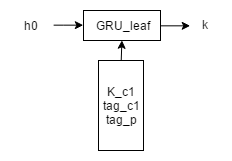
\includegraphics[width=0.4\linewidth]{figure/gruleaf}
    \begin{tikzpicture}
    \node(h)[io]{$h_{0}$};
    \node(gru)[process, right of=h, xshift=1cm]{GRU leaf};
    \node(k)[io, right of=gru, xshift=1cm]{k};
    \node(gruin)[process, below of=gru, yshift=-1cm, text width=1cm ]{$k_{c1}$ $tag_{c1}$ $tag_{p}$};
    \draw [arrow](h) -- (gru);
    \draw [arrow](gru) -- (k);
    \draw [arrow](gruin) -- (gru);
    \end{tikzpicture}
    \caption[Constituency TE-Tree-GRU leaf case]{Constituency TE-Tree-GRU leaf case}
    \label{fig:gruleaf}
\end{figure}



\subsubsection{Dependency TE-Tree-GRU} \label{sec:VTtreeDependency}
We built a model similar to constituency case. 
However, we did not put the parent node at the end of the chain. 
Instead, the parent node and its child nodes were sorted according to their position in the sentence. 
For any child node, the presentation vector \(k\), embedding vectors of POS-tag and dependency relationship type ares inputs for GRU timestep. 
At the parent node, dependency relationship type is set to 'self' and the temporal presentation vector \(k\) set to zeros vector. 
We took hidden state of the last time step as presentation vector \(k\) for parent node. 
In case of leaf node, we treated it as parent node without children. 
We built GRU chain with only parent node for leaf case. 
Fig.\ref{fig:dependencyvtgru} illustrates Dependency TE GRU model.

\begin{figure}[H]
    \centering
    % 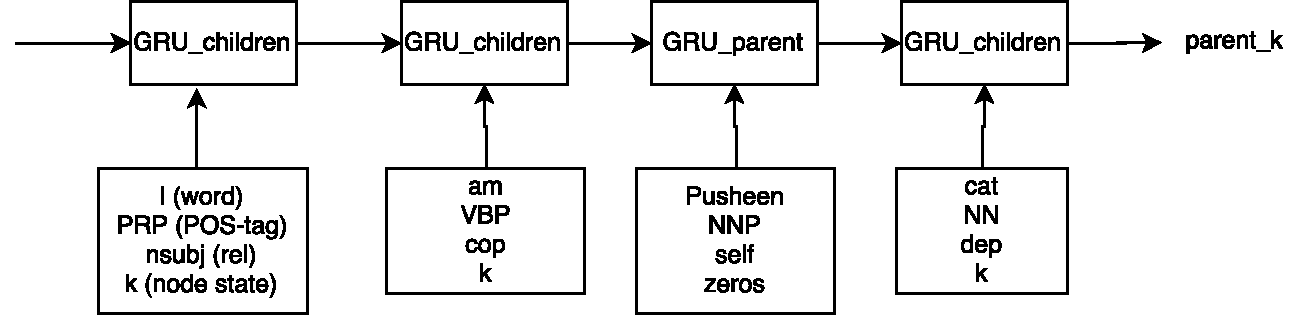
\includegraphics[width=0.9\linewidth]{figure/dependencyvtgru}
    \begin{tikzpicture}
\node(start)[io]{};
\node(gru1)[process, right of=start, xshift=1cm]{$GRU_{child}$};
\node(gruin1)[process, below of=gru1, yshift=-1cm, text width=3cm, align=center]{I (word) \\ PRP (POS-tag) \\ nsubj (rel) \\ k (node state)};

\node(gru2)[process, right of=gru1, xshift=2cm]{$GRU_{child}$};
\node(gruin2)[process, below of=gru2, yshift=-1cm, text width=1.5cm, align=center ]{am \\ VBP \\ cop \\ k};

\node(gru3)[process, right of=gru2, xshift=2cm]{$GRU_{parent}$};
\node(gruin3)[process, below of=gru3, yshift=-1cm, text width=1.5cm, align=center ]{Pusheen \\ NNP \\ self \\ zeros};

\node(gru4)[process, right of=gru3, xshift=2cm]{$GRU_{child}$};
\node(gruin4)[process, below of=gru4, yshift=-1cm, text width=1.5cm, align=center ]{cat \\ NN \\ dep \\ k};

\node(parentk)[io, right of=gru4, xshift=1cm]{$k_{parent}$};

% \node(gru5)[process, right of=gru4, xshift=1.5cm]{$GRU_{parent}$};
% \node(gruin5)[process, below of=gru5, yshift=-1cm, text width=1cm ]{$zeros$ $tag_{p}$ $tag_{p}$};

\draw [arrow](start) -- node(cat)[io,up,above]{$h_{0}$} (gru1); 
\draw [arrow](gru1) -- node(cat)[io,up,above]{$h_{1}$} (gru2); 
\draw [arrow](gru2) -- node(cat)[io,up,above]{$h_{2}$} (gru3); 
\draw [arrow](gru3) -- node(cat)[io,up,above]{$h_{3}$} (gru4);
% \draw [arrow](gru4) -- node(cat)[io,above]{$h_{4}$} (gru5);
\draw [arrow](gru4) -- (parentk);

\draw [arrow](gruin1) -- (gru1);
\draw [arrow](gruin2) -- (gru2);
\draw [arrow](gruin3) -- (gru3);
\draw [arrow](gruin4) -- (gru4);

% \draw [arrow](gruin5) -- (gru5);
    
    \end{tikzpicture}
    \caption[Dependency TE-Tree-GRU]{Dependency TE-Tree-GRU}
    \label{fig:dependencyvtgru}
\end{figure}

\subsubsection{Output layer and loss function}
We used softmax classifier and cross entropy loss function.  
For each node which has sentiment label, we used the vector presentation $k$ of that node as input to output layer and calculate loss against the given label. 
Root node's vector presentation $k$ was used to determine the sentiment class of whole sentences.

\hypertarget{sec:Glove-Amazon}{\section{Training Glove embedding on Amazon reviews dataset}}
\label{sec:gloveamazone}
Steps for preprocessing Amazon dataset for training word vectors on Glove:
\begin{enumerate}
\item For retraining Glove vectors, we only used Amazon Movies and TV reviews dataset (7,850,072 reviews)~\cite{mcauley2013hidden}, Amazon Book reviews(22,507,155 reviews) and new Movies and TV dataset (4,607,047 reviews)~\cite{McAuleyTSH15}~\cite{HeM16}.
\item All the reviews were grouped by product-ID ("asin" keyword in the \hyperref[sec:amazon]{JSON schema of the dataset}).
\item In each product-ID group, the reviews were sorted increasingly by their rating ("overall" keyword in the JSON schema of the dataset).
\item All the reviews were dumped into a plain text file.
\item The text file produced from the previous step was tokenized using Stanford Tokenizer~\cite{tokenizerpart}.
\end{enumerate}

The reason for doing step 2 and step 3 is because there is no definition of end-of-document in Glove model, which means words which appear in the beginning part of a document will be included in the context of words in the last part of the previous document, this lead to noise in training data, step 2 and 3 help us to mitigate this problem.

We named this word embeddings Glove Amazon.
For evaluating, we used Glove Amazon to replace Glove Common Crawl for initializing word embedding layer of Tree-LSTM.
Apart from that, the whole training process and hyper-parameters are kept unchanged (Sec.\ref{sec:treelstm}).

\hypertarget{sec:CNNtree}{\section{Combining Recursive Neural Networks with Convolution Neural Networks}}\label{sec:CNNtree}
\subsection{Model description}
\begin{figure}[H]
    \centering
    % 
\includegraphics[width=0.8\linewidth]{figure/convtreelstmsummary}
    % Convolution Tree-LSTM overview
    \begin{tikzpicture}
\node (input)[io]{input};
\node (emb)[process, right of=input, xshift=1.5cm, text width=2cm]{Embedding Layer};
\node (conv)[process, right of=emb, xshift=2cm, text width=2cm]{Convolution Layer};
\node (treelstm)[process, right of=conv, xshift=2cm]{Tree-LSTM};
\node (outputlayer)[process, right of=treelstm, xshift=2cm, text width=2.2cm]{Output Layer};
\node (output)[io, right of=outputlayer, xshift=1.5cm]{sentiment};

\draw [arrow](input)--(emb);
\draw [arrow](emb)--(conv);
\draw [arrow](conv) -- (treelstm);
\draw [arrow](treelstm) -- (outputlayer);
\draw [arrow](outputlayer) -- (output);
    \end{tikzpicture}
    \caption[Convolution Tree-LSTM overview]{Convolution Tree-LSTM overview}
    \label{fig:convtreelstmsummary}
\end{figure}
For this approach, we do experiment with two network architects:
\begin{description}
\item[CNN Tree-LSTM] Given the Constituency Tree-LSTM architect described in Sec.\ref{sec:treelstm},  we inserted a convolution layer between the word embedding layer and the Tree-LSTM's leaf-module.
The rest of TreeLSTM implementation was kept unchanged.
A diagram of CNN Tree-LSTM's modules can be found in Fig.\ref{fig:convtreelstmsummary}.
\item[CNN LSTM] Similar CNN Tree-LSTM but the Tree-LSTM module is replaced by a LSTM.\footnote{Although CNN LSTM seems similar to \hyperref[cnn-rnn]{CNN-RNN}~\cite{cnn-rnn}, we extended it for multichannel input and unsupervised pre-train it. We will explain these techniques in more details in Sec.\ref{sec:model-enhan}}
One advantage of CNN-LSTM compared to CNN Tree-LSTM is that CNN-LSTM can be unsupervised pre-trained as Language Model, while CNN Tree-LSTM can not (Sec.\ref{sec:unsupervised-pretrain}).
\end{description}

\subsubsection{Convolution layer} \label{sec:conv1c}
Our implementation is based on the convolution layer described in Sec.\ref{kim-cnn}.
\paragraph{Matrix presentation of sequences of words}
Given any sentence \(s\) of length \(n\), we denote \(x_i \in \mathbb{R}^d\) as a vector presentation of word-\(i\)th in the sentence.
Note that the first word in a sentence is word-\(0\)th, if the sentence is padded with dummy words on its left, these padded dummy words are indexed by negative integers.
Any sequence of words in the sentence which start at word-\(i\)th and end at word-\(j\)th can be presented as the following:
\begin{align}
    X_{i:j} &= x_i \oplus x_{i+1} \oplus ... \oplus x_{j} &\label{concat}
\end{align}
In Eq.\eqref{concat}, \(\oplus\) is concatenation operator which result in the matrix \(X_{i:j} \in \mathbb{R}^{d \times (j-i+1)}\).

\paragraph{Convolution filter}
Given that \(F\) is the set of all filters of the convolution layer, for any filter \(v \in F\) which has window size \(l\) and set of parameters \(\theta^{(v)} = \{ W^{(v)}, b^{(v)} | W^{(v)} \in \mathbb{R}^{d \times l}, b^{(v)} \in \mathbb{R}\}\), filter \({v}\) is applied on any sequence of word-\(i\)th to word-\((i+l-1)\)th through the following equation:
\begin{align}
    c^{(v)}_j &= f(W^{(v)} \otimes X_{i:i+l-1} + b^{(v)}) &\label{filter}
\end{align}

In Eq.\eqref{filter}, operator \(\otimes\) is the Hadamard product~\cite{element-prod}.  
\(b \in \mathbb{R}\) as bias term and \(f\) is an activation function.
For indexing, \(j = i + x\) with \(x \in \mathbb{N}\) and \(0 \leq x < l\).
If half-padding policy is employed then \(j = i + \floor{\frac{l}{2}}\).
For the case of multichannel input, given that the sentence is presented by any set of input channels \(Z\).
We will modify Eq.\eqref{filter} as follow:
\begin{align}
    \forall h \in Z, \; \; \hat{c}^{(v)}_{jh} &= f(W^{(v)} \otimes X_{i:i+l-1} + b^{(v)})& \\
    c^{(v)}_j &= \sum_{h \in Z} \hat{c}^{(v)}_{jh}&
\end{align}

By slicing the filter \(v\) through the sentence (i.e. applying the filter \(v\) on different sequences of length \(l\) along the sentence) we can get vector \(c^{(v)} = [c^{(v)}_0, c^{(v)}_1~\cdots]\) which is a feature map of the sentence \(s\).

\begin{figure}[H]
    \centering
    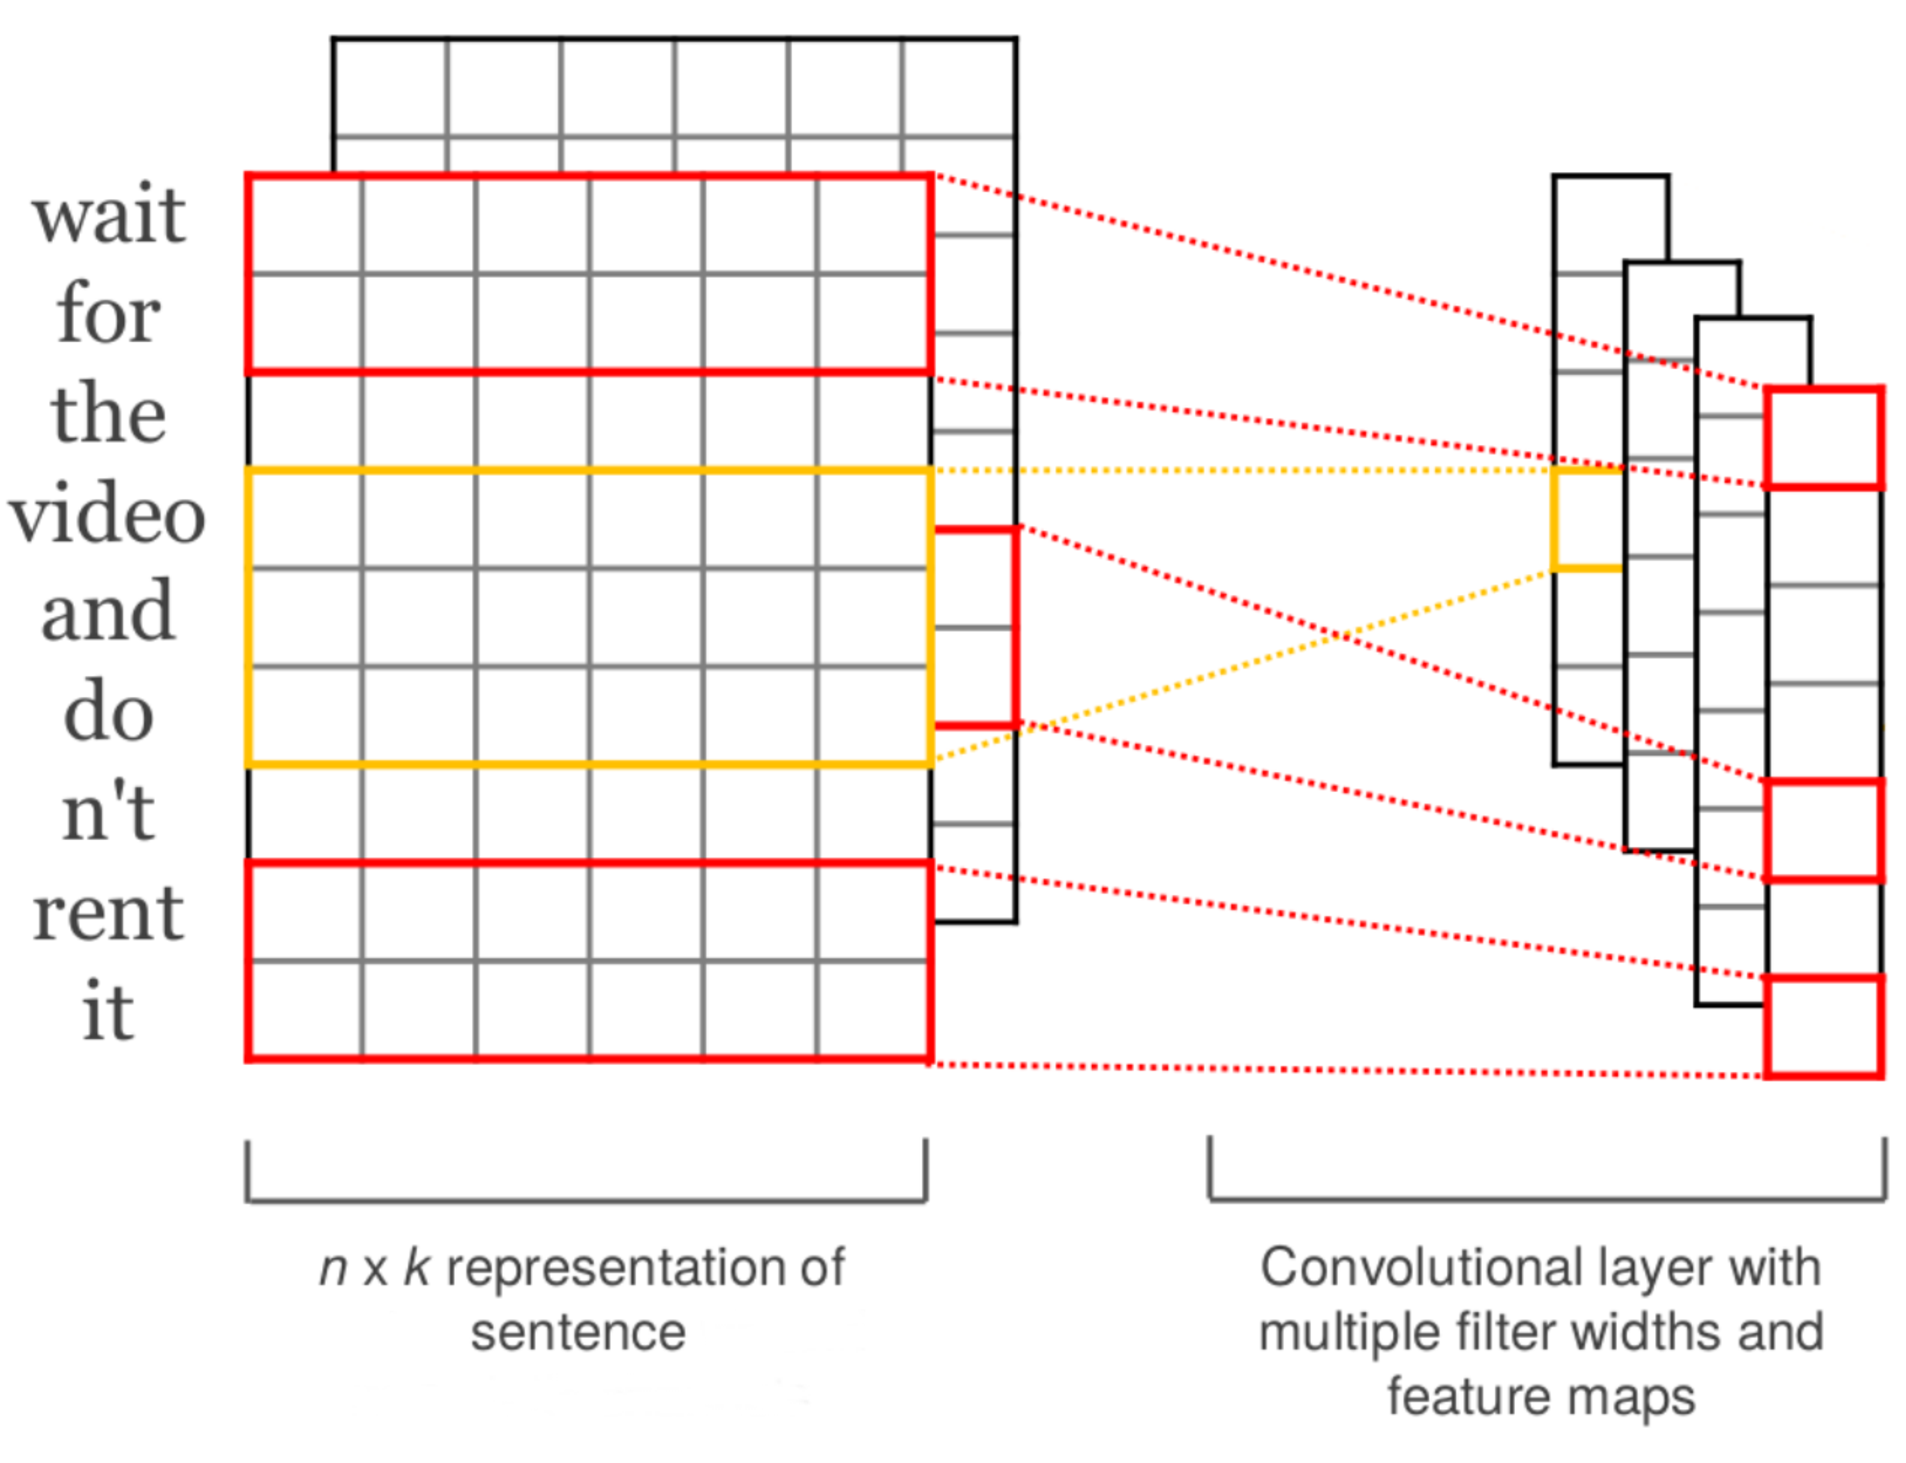
\includegraphics[scale=0.3]{figure/cnn-module}
    \caption[Convolution layer with two input channels]{Convolution layer with two input channels}
    \label{fig:cnn-module}
\end{figure}

Until now, we have not define the length of the feature map \(c^{(v)}\). 
To be able to work with Tree-LSTM (which required tree-structured inputs), all the feature maps produced by the convolution layer need to have length equal to that of the sentence \(s\) (which is \(n\) in this case).
For satisfying this constraint, all filters in \(F\) are restricted to have odd window sizes and being applied on the sentence according to half padding, unit strides policy~\cite{conv-arith}.
These conditions entail \({\forall u \in F,  c^{(u)} \in \mathbb{R}^n}\)~\cite{conv-arith}.
We demonstrate this policy in Fig.\ref{fig:half-padding}.

\begin{figure}[H]
    \centering
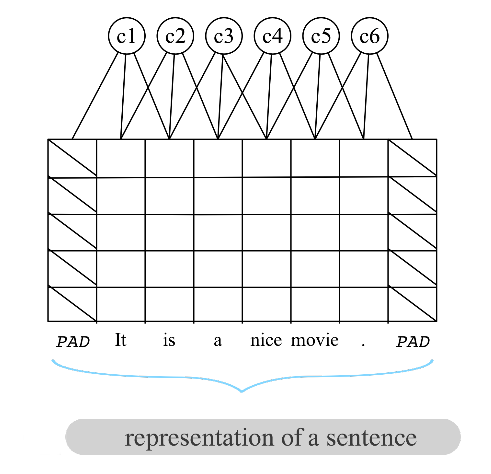
\includegraphics[scale=0.45]{figure/half-padding}
    \caption[Half padding, unit strides policy]{A convolution filter with window size 3 applying on a sentence according to half padding, unit strides policy.
    The length of the resulted feature map is equal to that of the sentence.}
    \label{fig:half-padding}
\end{figure}

Suppose the size of set of filters \(F\) is \(m\), all the feature maps produced by the set of filters is then concatenated into one matrix \(P \in \mathbb{R}^{m \times n}\), which each of its row is a feature maps.
After that, the column vectors of \(P\) are treated as input vectors for Tree-LSTM or any Recurrent Neural Network (Sec.\ref{sec:RNN}).

\subsubsection{Constituency Tree-LSTM module}
For this module, we reused Constituency Tree-LSTM~\cite{treeLSTM}.
Let \(d\) be the size of the input vectors, \(r
\) be the size of the memory cell and \(z\) be the number of sentiment classes. 

\paragraph{Leaf module}
Given any input vector \(x \in \mathbb{R}^d\), the calculation steps inside the leaf module can be expressed as follow:
\begin{align}
    o &= \sigma{\left( W^{(o)} x + a^{\left(o\right)}\right)} & \\
       c &= W^{(c)} x + a^{(c)} & \\
    h &= o \odot \tanh{\left(c\right)} &
\end{align}

In this module, \(W^{(o)}, W^{(c)} \in \mathbb{R}^{r \times d}\) and \(a^{\left(o\right)}, a^{(c)} \in \mathbb{R}^r\).

\paragraph{Composer module}
Given the input vectors \({h_l}\), \({c_l}\) from the left child node and \({h_r}\), \({c_r}\) from the right child node, the calculation steps inside the composer module can be expressed as follow:
\begin{align}
      i &= \sigma{ \left(U_l^{(i)} h_{l} + U_r^{(i)} h_{r} + b^{(i)} \right) } &\\
      f_{l} &= \sigma{\left(U_{l}^{(l)} h_{l} + U_{r}^{(l)} h_{r} + b^{(f)}\right)} & \\
      f_{r} &= \sigma{\left(U_{l}^{(r)} h_{l} + U_{r}^{(r)} h_{r} + b^{(f)}\right)} & \\
      o &= \sigma{\left( U_l^{(o)} h_{l} + U_r^{(o)} h_{r} + b^{(o)}\right)} &\\
      u &= \tanh{\left( U_l^{(u)} h_{l} + U_r^{(u)} h_{r} + b^{(u)}\right)} &\\
       c &= i \odot u + f_{l} \odot c_{l} + f_{r} \odot c_{r} & \\
    h &= o \odot \tanh{\left(c\right)} &
\end{align}

In this module, for any \(j \in \{i, l, r, o, u\}\) and \(x \in \{\l, r\}\), \(U_x^{(j)} \in \mathbb{R}^{r \times r}\) and \( b^{(j)} \in \mathbb{R}^r\).

\paragraph{Output module} Denoting sequence of words spanned by a sub-tree rooted at node \({j}\) as \({\{x\}_j}\).
Given \({h_j}\) is the \({h}\) ouput of node \({j}\), the prediction at node \({j}\) can be computed by the output module as follow:
\begin{align}
      \hat{p_{\theta}}(y \mid \{x\}_j ) &= softmax( W^{(s)} h_j + b^{(s)}) & \\
      \hat{y_j} &= \underset{y}{\mathrm{argmax}} \; \hat{p_{\theta}}(y \mid \{x\}_j ) &
\end{align}

In this module, for any \(W^{(s)} \in \mathbb{R}^{z \times r}\) and \( b^{(s)} \in \mathbb{R}^z\).
For loss function, negative log-likelihood with \(L2\) regularization was used.

\paragraph{Composing sentence}
Given any sentence \({s}\) of length \({n}\) and its parse tree, originally, Tree-LSTM composes the output vectors by first applying its leaf module on each word vectors then applying its composition function at each node of the parse tree in a bottom-up manner.
The output module is applied at the output \({h}\) of each node which has a sentiment label.

In case convolution layer was added, the only different is that for all \(0 \leq i \leq n-1\), the vector presentation of the word-\({i}\)th is replaced with the \({i}\)th-column of the matrix \({P}\) produced by the convolution layer.
This mean the size of input vectors \(d\) is equal to the number of filters \(m\).
 
\subsection{Models enhancements}\label{sec:model-enhan}
\subsubsection{Training Glove embedding on Amazon reviews dataset}\label{sec:reuse-glove-amazon}
We reused Glove Amazon word embedding (Sec.\ref{sec:gloveamazone}).

\subsubsection{Using multi-channel word embeddings}\label{sec:enhan-multi-channel}
This method was introduced by Yoon Kim~\cite{KimCNN}.
The description and analysis of this method can be found in Sec.\ref{kim-cnn}.
Although in his paper, in the training process of his 2-channel-CNN, Kim updated one channel and kept the other unchanged, we are not restricted ourselves to this rule.
The type of word embeddings used in each channel, the number of channels and the method for updating each channel are treated as hyper-parameters.

This method allows multiple parallel embedding layers in our model.
In other words, each word is presented by multiple vector representations.

\begin{figure}[H]
    \centering
    % 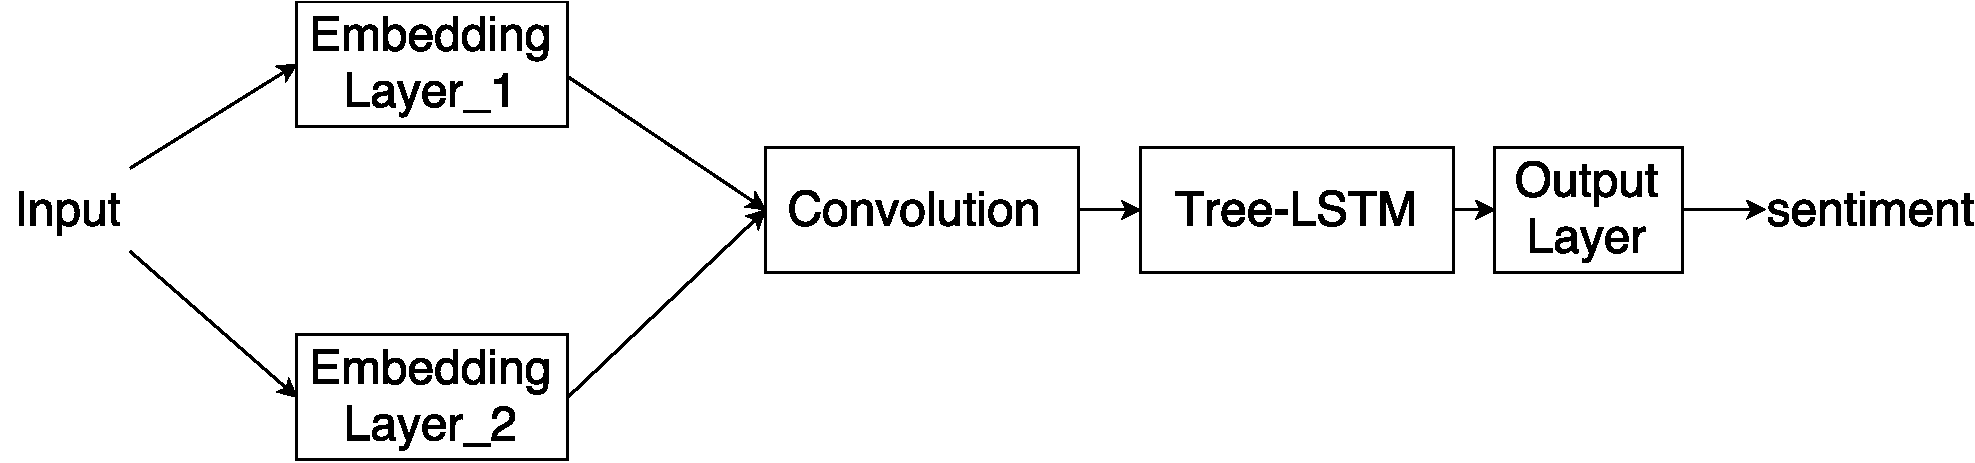
\includegraphics[width=0.8\linewidth]{figure/multichannelcnnlstm}
    \begin{tikzpicture}
    \node (input)[io]{input};
    \node (holder)[io, right of=input, xshift=1.5cm, text width=2cm]{};
    \node (emb1)[process, right of=input, xshift=1.5cm, yshift=1.5cm, text width=2cm]{Embedding Layer 1};
    \node (emb2)[process, right of=input, xshift=1.5cm, yshift=- 1.5cm, text width=2cm]{Embedding Layer 2};
    \node (conv)[process, right of=holder, xshift=2cm, text width=2cm]{Convolution Layer};
    \node (treelstm)[process, right of=conv, xshift=2cm, text width=2cm]{Tree-LSTM};
    \node (outputlayer)[process, right of=treelstm, xshift=2cm, text width=2.2cm]{Output Layer};
    \node (output)[io, right of=outputlayer, xshift=1.5cm]{sentiment};
    
    \draw [arrow](input)--(emb1);
    \draw [arrow](input)--(emb2);
    \draw [arrow](emb1)--(conv);
    \draw [arrow](emb2)--(conv);
    \draw [arrow](conv) -- (treelstm);
    \draw [arrow](treelstm) -- (outputlayer);
    \draw [arrow](outputlayer) -- (output);
    \end{tikzpicture}
    \caption[Convolution Tree-LSTM overview]{Two input channel Convolution Tree-LSTM overview}
    \label{fig:multichannelcnnlstm}
\end{figure}


\subsubsection{Pre-training models on Amazon reviews dataset}
\label{enhan-unsupervised-pretrain}
We presented several methods for unsupervised pre-training neural network models and given some hypotheses on the beneficial effects of these methods in Sec.\ref{sec:unsupervised-pretrain}.
\paragraph{Steps for preprocessing Amazon dataset for training Language Model}
\label{sec:preprocessamazonglove-LM}
\begin{enumerate}
\item For retraining Glove vectors, we only used new Movies and TV dataset (4,607,047 reviews)~\cite{McAuleyTSH15}~\cite{HeM16}.
\item All the reviews were grouped by product-ID ("asin" keyword in the \hyperref[sec:amazon]{JSON schema of the dataset}).
\item In each product-ID group, the reviews were sorted increasingly by their rating ("overall" keyword in the JSON schema of the dataset).
\item A special character sequence was added at the end of each review to mark its end.
After that, all the reviews were dumped into a plain text file.
\item The text file produced from the previous step was tokenized using Stanford Tokenizer~\cite{tokenizerpart}.
\item The tokenized text file was then divided into training and test set using 95:5 split.
As this is a pre-training process, we used only 5\% of the data to test if the Language Model was trained properly.
\end{enumerate}

Step 2, 3 and 4 are for mitigating the problem of noise in training data which have been presented in Sec.\ref{sec:gloveamazone}.